% ============================================================================
% DHG508 期末設計論文（中文版）— zhanguo_qunxiong
% 編譯：XeLaTeX → Biber → XeLaTeX ×2
% ============================================================================

\documentclass[12pt,a4paper]{article}

\usepackage{fontspec}
\newcommand{\MainLatinFont}{Times New Roman}
\newcommand{\FallbackLatinFont}{TeX Gyre Termes}
\newcommand{\MainCJKFont}{Noto Serif CJK TC}
\newcommand{\FallbackCJKFont}{FandolSong-Regular.otf}

\IfFontExistsTF{\MainLatinFont}
  {\setmainfont{\MainLatinFont}}
  {\setmainfont{\FallbackLatinFont}}

\usepackage{xeCJK}
\IfFontExistsTF{\MainCJKFont}
  {\setCJKmainfont{\MainCJKFont}}
  {\IfFontExistsTF{Songti TC}
    {\setCJKmainfont{Songti TC}}
    {\IfFontExistsTF{PMingLiU}
      {\setCJKmainfont{PMingLiU}}
      {\setCJKmainfont{\FallbackCJKFont}}}}

\usepackage[a4paper, margin=1in]{geometry}
\usepackage{setspace}
\usepackage{booktabs}
\usepackage{array}
\usepackage{graphicx}
\usepackage{csquotes}

\usepackage[notes, backend=biber, autolang=other, isbn=false]{biblatex-chicago}
\addbibresource{references.bib}

\renewcommand{\footnotesize}{\fontsize{10}{12}\selectfont}
\usepackage[hidelinks]{hyperref}

\title{\textbf{知識即戰力：一款讓史料上臉的戰國群雄策略游戲}\\[0.3em]
\large 設計理據、證據邊界與復盤}
\author{James\\嶺南大學 $\cdot$ DHG508 批判性數字人文\\
\footnotesize 遊戲：\url{https://zhanguo-godot.zhanguo-godot.workers.dev}\\
\footnotesize 仓库：\url{https://github.com/wangsizhangyang-cloud/dhg508}}
\date{2026 年 11 月 25 日}

\begin{document}
\maketitle

\begin{abstract}
\noindent
本文介紹《戰國群雄》——一款以雲端部署的 Godot~4 戰國大戰略模擬。玩家執
七雄之一，通過國策樹、內政、外交與陣法戰鬥的 HOI4 式回合循環爭奪統一，
而屏幕上每一個數字都可溯源：資料層提取自《史記》《國語》《荀子》與法兵
文獻，每條主張標注\emph{據}（有文獻明文）、\emph{推斷}（由材料折算）或
\emph{設}（遊戲設計虛構），國策樹與法令節點在遊戲內直接引用出處。十七個
Godot 無頭自檢腳本與對兩個部署網址的 Playwright 端到端測試保證構建的誠
實。核心結論：一款戰略遊戲可以把史學書寫長在界面上——節點帶引文、證據
表列邊界——而絲毫不損害它作為遊戲的可玩性。
\end{abstract}

\onehalfspacing

\section{歷史問題與媒介}

本項目同時回答兩個問題。歷史問題：戰國——一個瘋狂變法、全民皆兵、外交
權謀的世界——作為一個\emph{系統}是怎樣運轉的？玩家能否親身體感這個系統？
設計問題隨之而來：一款大戰略遊戲能否做到屏幕上\emph{每一個}數字要麼有文
獻明文、要麼誠實標注為折算、要麼公開承認為虛構——而遊戲不會被自己的腳註
壓垮？

互動模擬是恰當的媒介，因為歷史問題的答案是系統性的。讀到「齊技擊不如魏
武卒，魏武卒不如秦銳士」\autocite{xunzi}，得到的是一個強弱序；只有親手
執秦與魏對抗，玩家才會為這個差距\emph{付代價}——在維持費裡、在招募成本
裡、在先打哪個省的取捨裡。遊戲把課程的核心主張操作化了：歷史知識應當是
\emph{可兌換的資產}——讀文獻不是遊戲旁邊的作業，而是你判斷先搶哪項變法、
先要哪個省的依據。

出貨版本是 Godot~4 版：87 省地圖上的完整征服遊戲，以 WebGL 構建部署，
任何人用瀏覽器即可打開。此前有一個 Web 規則原型作鋪墊；原型中搭建的教學
關與 LLM agent 未隨出貨版交付（見第~\ref{sec:postmortem}~節）。

\section{史料與學術對話}

一手語料是司馬遷《史記》——人物、戰績與諸國敘事的底本——以《國語》
\autocite{guoyu}互證，軍事組織方面以《荀子·議兵》及法兵文獻為據。局限如
實說明：這些是傳世文獻而非出土文獻；資料庫中 1215 條戰績做了完整性核驗
並與互證文獻抽樣比對，但未逐條重審；遊戲內中文引文採用通行篇章定位法，
不同版本頁碼或有出入。

三篇學術文獻構成設計對話的錨點。其一，Harnes 對四十一項實證研究的範圍
綜述指出：歷史共情是認知—情感複合體，\emph{實質知識}是前提，語境化與證
據工作才是真正的瓶頸\autocite{harnes2025empathy}。這為遊戲的核心機制提
供了依據：知識是結算項——解鎖改革、封鎖死路、進入戰鬥公式——而不是我們
奢望玩家自帶的前置條件。該綜述同時警告第一人称代入會加劇「以今非古」，
因此出貨版刻意不給玩家任何歷史化身。

其二，Park 等人的生成式 agent 架構展示了 LLM agent 如何維持記憶、感知
與行動——以及關鍵的一點：檢索會失敗、會編造\autocite{park2023generative}。
項目據此搭建了周幽王 agent，採用該設計最窄的可行切片：只從《周本紀》有
明文的事件手工策展記憶白名單、有界的感知窗口、以及經世界引擎校驗後才生
效的單動作 JSON 輸出契約。agent 可以在語氣上即興，不能在史實上即興。

其三，Zhang 對西周紀年的重新編年表明：前 771 年並非無爭議的錨點——即位
紀年可以另樣重構，771 本身即為可爭論之點\autocite{zhang2023chronology}。
遊戲不掩蓋這一點，而是在編年史與史料館中把爭議本身作為內容呈現：玩家消
化其史料批判卷宗後會明白，自己正在玩的這套曆法本身就是一場論辯。

\section{架構與邊界}

系統分層，讓機器而不只讓人可以核驗歷史內容。\textbf{資料層}（JSON，由
共享 SQLite 源經導出腳本生成）收錄 190 位武將及其 1215 條帶
\texttt{original\_text} 與出處的戰績；由文獻比較句轉換的 15 個兵種與 13
條克制關係；以譚其驤歷史地圖集上真實經緯城邑為錨點的 87 省
\autocite{tan1982atlas}；以及官員名錄。\textbf{規則層}（GDScript）以戰
鬥公式解算回合循環——收入、訓練、下令、圍城、事件——公式消費兵種構成、
克制、地形、城防、將領與四種陣形（橫陣、錐形、方圓、箭矢）。\textbf{戰
略層}承載 HOI4 式國策樹，枝幹按諸子學派（法、兵、農、基建）展開，每個
節點引用出處——秦系統之根引用《史記》記獻公之志，「農戰之法」引用《商君
書》。\textbf{外交層}處理條約、調停與談判，小國依利益而非腳本忠誠行事。

部署為靜態 Godot~4 WebGL 導出，前置一個小型 Cloudflare Worker：Worker
將 \texttt{/} 以 302 跳轉到 no-store 的啟動頁（繞開邊緣緩存舊構建），再
按 \texttt{Accept-Encoding} 在邊緣壓縮流式傳輸 \texttt{index3.wasm} 與
\texttt{index3.pck}；GitHub Pages 鏡像提供未壓縮原件。認知邊界既是時間
的也是結構的：資料層不含前 221 年統一之後的任何事件，遊戲的虛構部分——
公式、陣形數值、地圖幾何——在下表標為\emph{設}。標注體系循課程通例：
\emph{據}有明文、\emph{推斷}由材料折算、\emph{設}為設計虛構。

有一個範圍決定值得寫在正文而非腳註裡：教學關與 LLM 周幽王 agent 已在
Web 原型中建成並通過驗證，但最終封版交付的 Godot 構建\emph{不含}它們。
它沉澱下的設計原則延續下來——記憶白名單、輸出校驗、以及拒絕讓玩家佔有歷
史人物的第一人称——但公開網址刻意是一款通過事件、編年與引文改革去「遇
見」過去的遊戲，而非通過聊天窗口。凍結範圍與非目標記錄於
\texttt{docs/plan.md}；圖~\ref{fig:schematic} 總結架構分層及各層對應的
證據等級。

\begin{figure}[htbp]
  \centering
  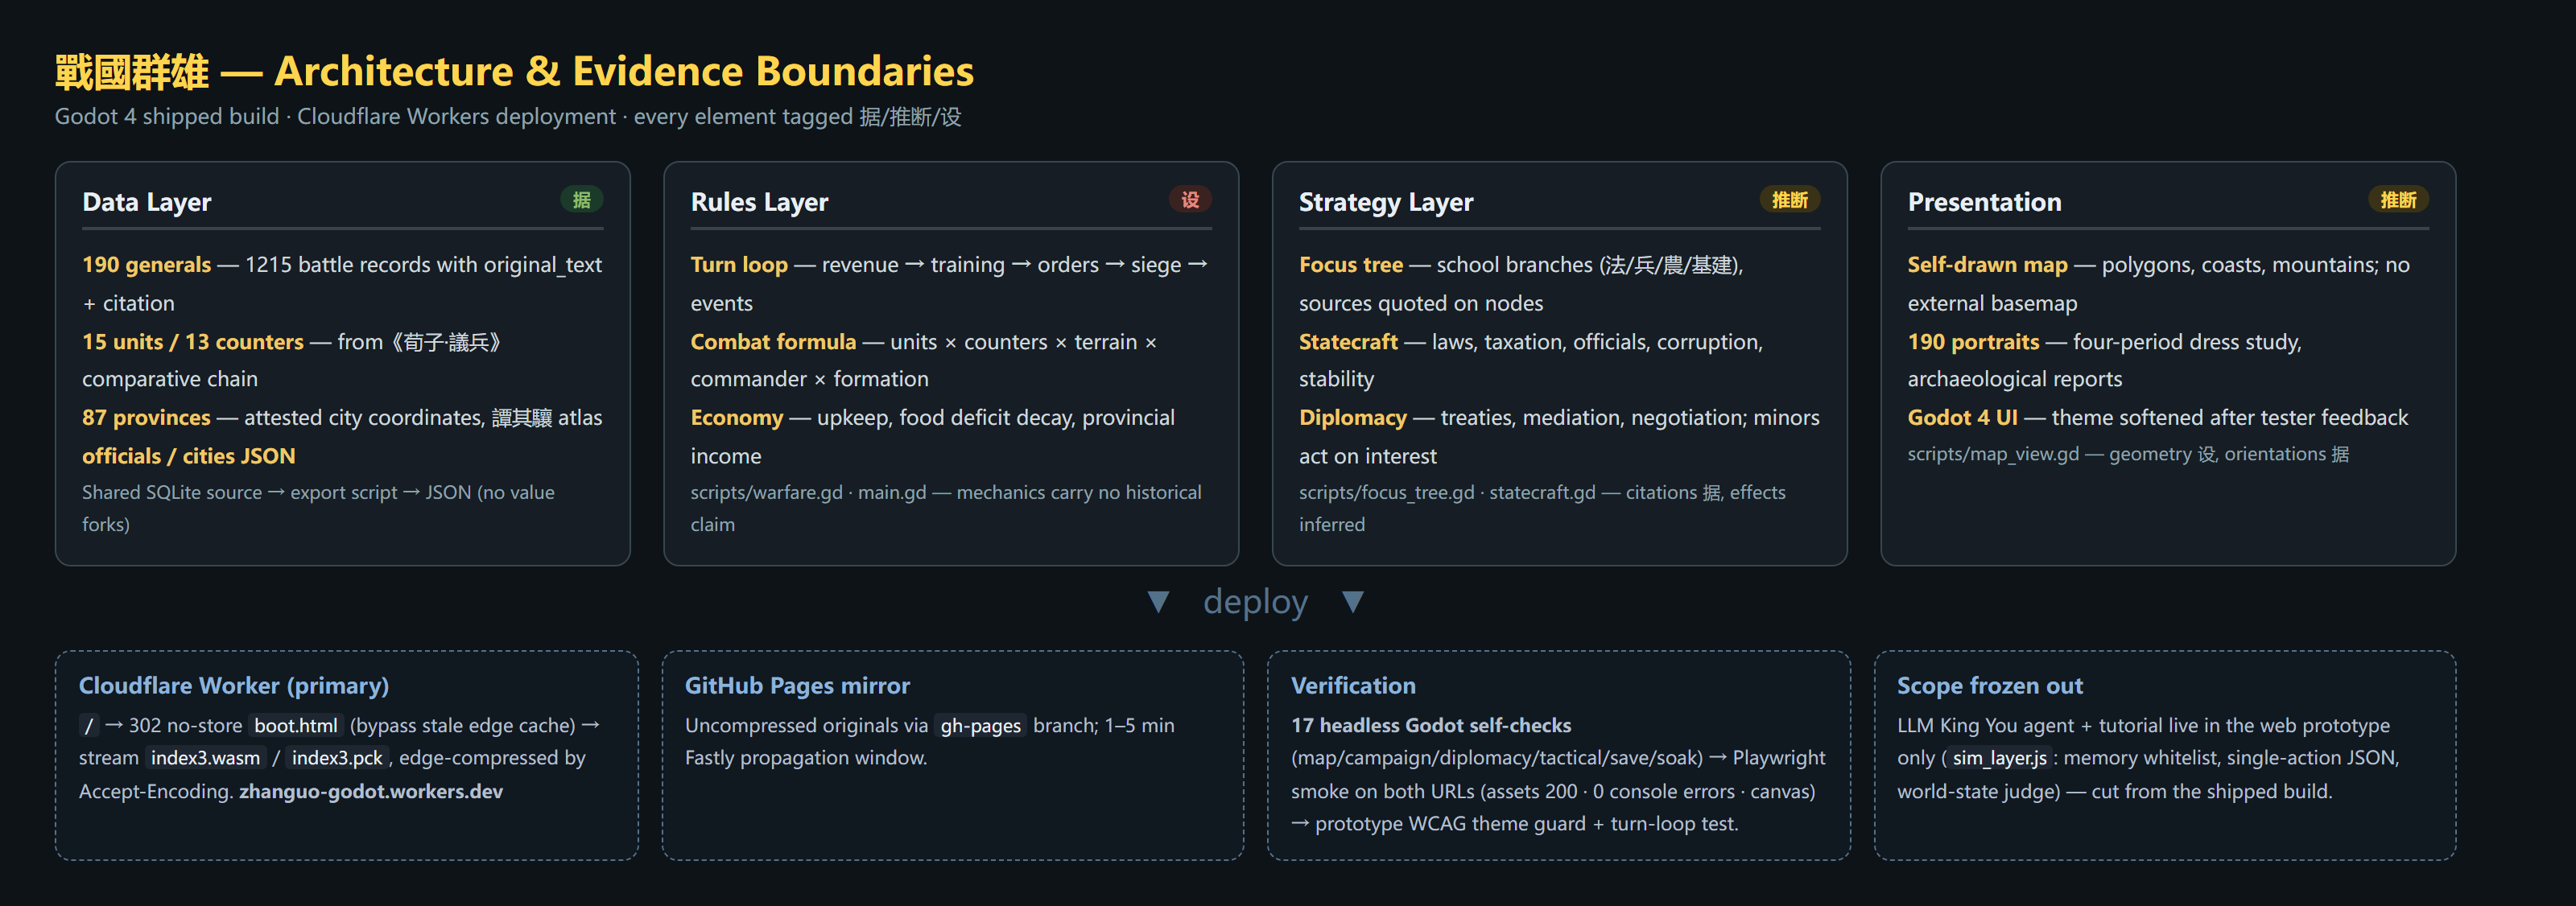
\includegraphics[width=0.86\textwidth]{schematic.png}
  \caption{《戰國群雄》架構：資料、規則、戰略、呈現四層；部署與驗證路徑；
  以及各層標注的證據等級（\emph{據}有明文、\emph{推斷}折算、\emph{設}虛構）。}
  \label{fig:schematic}
\end{figure}

\section{證據表}

表~\ref{tab:evidence} 由 \texttt{evidence.csv} 經
\texttt{make\_evidence\_table.py} 自動生成；LaTeX 表格永不手改。

\begin{table}[htbp]
  \centering
  \scriptsize
  \singlespacing
  \renewcommand{\arraystretch}{2.2}
  \setlength{\extrarowheight}{2pt}
  % Auto-generated from evidence.csv by make_evidence_table.py — edit the CSV, not this file.
\begin{tabular}{p{0.27\textwidth}p{0.20\textwidth}p{0.13\textwidth}p{0.08\textwidth}p{0.22\textwidth}}
  \toprule
  \textbf{Claim / Element} & \textbf{Source / File} & \textbf{Locator} & \textbf{Level} & \textbf{Boundary / Limit} \\
  \midrule
  Deposition of Queen Shen and Crown Prince Yijiu; Marquis of Shen allies with Zeng and the Quanrong; You is killed at the foot of Mount Li & Sima Qian, Shiji, 'Zhou benji' and 'Qin benji' & Shiji 4.149; Shiji 5.179 & 据 & Received text accepted for teaching; variant accounts exist \\
  The beacon-fire episode: You lights the beacons but the lords no longer come & Shiji, 'Zhou benji' & Shiji 4.147-148 & 据 & Received-text narrative; later scholarship questions its historicity \\
  Duke Xiang of Qin escorts Prince Ping east and is enfeoffed as a hou west of the Qi river & Shiji, 'Qin benji' & Shiji 5.179 & 据 & Boundary of the grant ('Qi between the rivers') is summarized from the text \\
  Bo Yangfu and Shi Bo foresee the fall of Western Zhou & Guoyu, 'Zhou yu xia' and 'Zheng yu' & Guoyu 1; Guoyu 16 & 据 & Dialogue is a received literary composition \\
  'Qi hired retainers are no match for Wei's wuzu; Wei's wuzu are no match for Qin's ruishi' -> counter chain of unit types & Xunzi, 'Yi bing' & Xunzi 15 & 据 & The comparative sentence is quoted; the numeric combat coefficients are our conversion \\
  Focus-tree and law nodes carry their sources inside the game (e.g. 'Agronomy and War' quotes the Shang jun shu) & node 'cite' fields in scripts/focus\_tree.gd and scripts/statecraft.gd & scripts/focus\_tree.gd & 推断 & The quoted sources are real; the node effects are game balance \\
  Province anchors use historically attested cities with real coordinates & Tan Qixiang, Zhongguo lishi ditu ji, Warring States sheets & data/provinces.json & 推断 & Some city locations are scholarly conjectures; coordinates digitized by eye from the atlas \\
  Map geometry: province polygons & coastline and mountain polylines & self-drawn vector data rendered by MapView & scripts/map\_view.gd & 设 \\
  Six-stat values for 190 generals & battle records weighted with Shiji verdicts & data/generals.json & 推断 & Derived numbers; rationale recorded but the scale is ours \\
  Formation system (line/wedge/square/arrow) from ancient military practice & Zhoubing texts; game balance & scripts/warfare.gd & 设 & Named formations are attested; the numeric modifiers are invented \\
  King You agent with memory whitelist and one-action JSON (web prototype only) & Park et al. 2023 memory-stream design; Shiji 'Zhou benji' events & prototype sim\_layer.js & 推断 & Built and verified in the prototype; cut from the shipped Godot build at the scope freeze \\
  Round economy & upkeep and combat resolution formula & game rules engine & scripts/warfare.gd + scripts/main.gd & 设 \\
  771 BCE is not the undisputed year of the fall of Western Zhou & Zhang 2023 re-dating of the Zhou accession chronology & Zhang 2023 pp. 18-19 & 据 & Presented as an optional intelligence layer \\
  \bottomrule
\end{tabular}

  \caption{主張與設計要素的出處、證據等級（\emph{據}明文、\emph{推斷}折
  算、\emph{設}虛構）與邊界。}
  \label{tab:evidence}
\end{table}

\section{驗證與真人測試}

驗證分層，使失敗廉價、定位精準。第一層是十七個 Godot 無頭自檢腳本，對真
實引擎二進制運行——地圖連通、戰役流程、奪城、兵團合併、外交與調停、談
判、官員、百家、國策樹、戰術戰鬥、關隘通道、存讀檔、結局、敗北與多回合
壓測——提交前全部必須 PASS。第二層對導出的 Web 構建做端到端檢查：
Playwright 冒煙套件加載兩個部署網址（Cloudflare Workers 與 GitHub
Pages），斷言每個關鍵資產（\texttt{boot.html}、\texttt{index3.js}、
\texttt{index3.wasm}、\texttt{index3.pck}）返回~200，等待軟件渲染下的
啟動完成，並要求零控制台錯誤與 canvas 正常呈現。Web 原型另配有 WCAG 配
色對比護欄與回合循環交互測試，均為回應測試者反饋而加。

兩位外部測試者在自己的設備上使用了構建。他們的反饋務實而不戲劇化，兩個
問題都已修復並鎖定。第一位抱怨字體顏色與背景幾分鐘後就覺得刺眼；配色重
構以柔化深色面板上的文字對比，且對比檢查現已護住主題，刺眼組合無法回歸。
第二位覺得操作繁瑣——移動軍隊與確認回合點擊太多；調兵與回合確認流程已
精簡為更少的合併操作，鍵盤快捷鍵（空格結束回合）提升為一等公民並有回歸
測試覆蓋。兩項修復都以永久測試存在，投訴過的問題不會悄悄復發。完整反饋
記錄見 \texttt{docs/user-feedback.md}。

\section{復盤（Post-Mortem）}
\label{sec:postmortem}

\begin{enumerate}
  \item \textbf{有效的部分。}早期把學術文獻轉成設計約束——Harnes 對教學、
  Park 對 agent 架構、Zhang 對紀年——此後每場爭論都能靠指一個頁碼而非靠
  直覺解決。單一真相源的資料管線物有所值：Godot 構建消費導出的 JSON，數
  值不會在原型與出貨版之間分叉。無頭引擎測試在任何玩家看到之前就攔住了
  地圖與規則回歸；流式邊緣壓縮讓 WebGL 構建的加載可以忍受。
  \item \textbf{失敗的部分。}原型幽王 agent 在用戶故意誘導下洩漏未來歷
  史；輸入側的提示詞約束在蓄意攻擊面前毫無價值，修復靠的是世界狀態校驗
  器。首發界面本身就是測試者發現的失敗：刺眼的配色與繁瑣的操作——初版
  把這些當成外觀瑕疵而非設計缺陷。生成的立繪雖在服制上有考古依據，但
  190 張之間藝術風格漂移——尚未解決的一致性問題。
  \item \textbf{改變的部分。}原計劃是開放沙盒加腳本化教學戰役和可對話的
  周幽王；封版交付的卻是更深、更可驗證的內核——國策樹、內政、外交、陣法
  ——落在 Godot 構建上，教學關與 agent 留在原型裡。周幽王的第一人称玩法
  早已依文獻中「以今非古」的警告被放棄，改為把他當作受約束的他者。水師
  移動與深度合縱連橫外交被明確延後。
  \item \textbf{局限與 AI 工具。}「知識即資產循環能\emph{提升學習}」仍是
  設計假設：未做前測/後測，文獻也不支持「遊戲普遍優於電影」的主張。地圖
  的 Voronoi 幾何不貼合歷史上要緊的陘口與河流，87 省經濟未做三十五回合
  以上的壓力測試。構建過程使用 Claude 與 GPT 級模型做資料提取與代碼輔助
  （每條引用經人工復核），立繪集使用圖像模型，原型 agent 由本地 LLM 驅動。
\end{enumerate}

\singlespacing
\footnotesize
\printbibliography[title={參考文獻}]

\end{document}
